\documentclass[11pt]{article}
\usepackage[letterpaper]{geometry}
\usepackage{MATH562}

\begin{document}
\noindent \textbf{\Large{Caleb Logemann \\
MATH 562 Numerical Analysis II \\
Final Exam
}}

%\lstinputlisting[language=Matlab]{H01_23.m}
\begin{enumerate}
    \item % #1 Done
        Let $A \in \RR^{m \times m}$ be written in the form $A = L + D + U$,
        where $L$ is strictly lower triangular, $D$ is the diagonal of $A$, and $U$
        is the strictly upper triangular part of $A$.
        Assuming $D$ is invertible, $A\v{x} = \v{b}$ is equivalent to
        $\v{x} = -D^{-1}\p{L + U}\v{x} + D^{-1}\v{b}$.
        The Jacobi iteration method for solving $A\v{x} = \v{b}$ is defined by
        \[
            \v{x}^{(n+1)} = -D^{-1}\p{L + U}\v{x}^{(n)} + D^{-1}\v{b}
        \]
        Show that if $A$ is nonsingular and strictly row diagonally dominant:
        \[
            0 < \sum{j \neq i}{}{\abs{a_{ij}}} < \abs{a_{ii}}
        \]
        then the Jacobi iteration converges to $\v{x}_* = A^{-1}\v{b}$ for each
        fixed $\v{b} \in \RR^m$.
        % Hint: the infinity norm is a convenient one to use

        \begin{proof}
            Let $\v{e}_n$ be the error of the nth iteration of the Jacobi iteration
            from the actual solution, that is let
            \[
                \v{e}_n = \v{x}^{(n)} - \v{x}_*.
            \]
            The Jacobi iteration converges to the real solution if
            \[
                \lim{n \to \infty}{\norm[\infty]{\v{e}_n}} = 0 
            \]
            The error vector can be expressed recursively by noting that
            $\v{x}^{(n)}$ is the Jacobi iteration evaluated on $\v{x}^{(n-1)}$
            and that $\v{x}_*$ is a fixed point of the Jacobi iteration as it is
            the true solution to the linear system.
            This means that
            \begin{align*}
                \v{x}^{(n)} &= -D^{-1}\p{L + U}\v{x}^{(n-1)} + D^{-1}\v{b} \\ 
                \v{x}_* &= -D^{-1}\p{L + U}\v{x}_* + D^{-1}\v{b}.
            \end{align*}
            Therefore we can express the error recursively as
            \begin{align*}
                \v{e}_n &= \v{x}^{(n)} - \v{x}_* \\
                \v{e}_n &= \p{-D^{-1}\p{L + U}\v{x}^{(n-1)} + D^{-1}\v{b}} - \p{-D^{-1}\p{L + U}\v{x}_* + D^{-1}\v{b}} \\
                \v{e}_n &= -D^{-1}\p{L + U}\v{x}^{(n-1)} + D^{-1}\p{L + U}\v{x}_* \\
                \v{e}_n &= -D^{-1}\p{L + U}\p{\v{x}^{(n-1)} - \v{x}_*} \\
                \v{e}_n &= -D^{-1}\p{L + U} \v{e}_{n-1}.
                \intertext{Extrapolating this backwards we see that $\v{e}_n$
                    can be expressed in terms of $\v{e}_0$}
                \v{e}_n &= \p{-D^{-1}\p{L + U}}^n \v{e}_{0}.
            \end{align*}
            Now we can consider the limit of $\norm[\infty]{\v{e}_n}$ as $n$
            goes to infinity.
            \begin{align*}
                \lim{n \to \infty}{\norm[\infty]{\v{e}_n}} &= \lim{n \to \infty}{\norm[\infty]{\p{-D^{-1}\p{L + U}}^n \v{e}_{0}}} \\
                \lim{n \to \infty}{\norm[\infty]{\v{e}_n}} &\le \norm[\infty]{\v{e}_{0}} \lim{n \to \infty}{\norm[\infty]{D^{-1}\p{L + U}}^n}
            \end{align*}
            Now consider $\norm[\infty]{D^{-1}\p{L + U}}$.
            The infinity norm is the max row sum of the matrix, that is
            \[
                \norm[\infty]{D^{-1}\p{L + U}} = \max*_{1 \le i \le m} \sum{j=1}{m}{\abs{\p{D^{-1}\p{L + U}}_{ij}}}
            \]
            Because $L + U = A - D$, $\p{L + U}_{ij} = a_{ij}$ if $i \neq j$ and $\p{L + U}_{ii} = 0$.
            Also $D^{-1}$ is diagonal with $\p{D^{-1}}_{ii} = \frac{1}{D_{ii}} = \frac{1}{a_{ii}}$.
            Therefore the matrix product $D^{-1}\p{L + U}$ has entries $\p{D^{-1}\p{L + U}}_{ij} = \frac{a_{ij}}{a_{ii}}$ if $i \neq j$ or 
            if $i = j$, then $\p{D^{-1}\p{L + U}}_{ii} = 0$.
            We can now say that
            \begin{align*}
                \norm[\infty]{D^{-1}\p{L + U}} &= \max*_{1 \le i \le m} \sum{j \neq k}{}{\abs{\frac{a_{ij}}{a_{ii}}}} \\
                \norm[\infty]{D^{-1}\p{L + U}} &= \max*_{1 \le i \le m} \frac{1}{\abs{a_{ii}}} \sum{j \neq k}{}{\abs{a_{ij}}}
                \intertext{However since $A$ is strictly row diagonally dominant $\abs{a_{ii}} > \sum{j \neq k}{}{\abs{a_{ij}}}$,
                    we can conclude that $\frac{1}{\abs{a_{ii}}} \sum{j \neq k}{}{\abs{a_{ij}}} < 1$. Therefore}
                \norm[\infty]{D^{-1}\p{L + U}} &< 1
            \end{align*}
            Since $\norm[\infty]{D^{-1}\p{L + U}} < 1$, it is true that
            $\lim{n \to \infty}{\norm[\infty]{D^{-1}\p{L + U}}^n} = 0$.
            Thus
            \begin{align*}
                \lim{n \to \infty}{\norm[\infty]{\v{e}_n}} &\le \norm[\infty]{\v{e}_{0}} \lim{n \to \infty}{\norm[\infty]{D^{-1}\p{L + U}}^n} \\
                \lim{n \to \infty}{\norm[\infty]{\v{e}_n}} &\le 0
            \end{align*}
            This shows that the error converges to zero, and this proves that
            the Jacobi iteration does converge to the true solution if $A$ is
            strictly row diagonally dominant.
        \end{proof}

    \item % #2
        Let $A \in \RR^{m \times m}$ be symmetric positive definite (SPD),
        $\v{b} \in \RR^m$ and define $\phi:\RR^m \to \RR$ by
        \[
            \phi(\v{x}) = \frac{1}{2}\v{x}^T A \v{x} - \v{x}^T \v{b}
        \]
        Suppose $K$ is a subspace of $\RR^m$.
        Show that $\hat{\v{x}} \in K$ minimizes $\phi(\v{x})$ over $K$ if and
        only if $\nabla \phi(\hat{\v{x}}) \perp K$.

        \begin{proof}
            
        \end{proof}

    \item % #3

    \item % #4
        Let $A \in \RR^{n \times n}$ be a symmetric positive definite matrix.
        Let Gaussian elimination be carried out on $A$ without pivoting.
        After $k$ steps, $A$ will be reduced to the form
        \[
            A^{(k)} =
            \begin{pmatrix}
                A_{11}^{(k)} & A_{12}^{(k)} \\
                0            & A_{22}^{(k)} \\
            \end{pmatrix}
        \]
        where $A_{22}^{(k)}$ is an $(n - k) \times (n - k)$ matrix.
        Show by induction
        \begin{enumerate}
            \item[(a)]
                $A_{22}^{(k)}$ is symmetric positive definite.

                \begin{proof}
                    
                \end{proof}

            \item[(b)]
                $a_{ii}^{(k)} \le a_{ii}^{(k-1)}$ for all $k \le i \le n$,
                $k = 1, \cdots, n - 1$.

                \begin{proof}
                    
                \end{proof}
        \end{enumerate}

    \item % #5
        Let $A \in \RR^{m \times n}$ with $m > n$ and
        \[
            A = 
            \begin{pmatrix}
                A_1 \\
                A_2
            \end{pmatrix}
        \]
        where $A_1$ is a nonsingular $n \times n$ matrix, and $A_2$ is an
        $(m - n) \times n$ arbitrary matrix.

    \item % #6
        Let $A \in \CC^{m \times m}$ with $\rank(A) = r$.
        Suppose an SVD of $A$ is given by $A = U\Sigma V^*$, where
        $\v{u}_1, \v{u}_2, \ldots, \v{u}_m$ denote the columns of $U$ and
        $\v{v}_1, \v{v}_2, \ldots, \v{v}_m$ denote the columns of $V$.
        Prove that $\langle\v{v}_{r+1}, \ldots, \v{v}_m\rangle = \null(A)$.

        \begin{proof}
            
        \end{proof}

    \item % #7
        Problem 33.2 (Page 255) 

    \item % #8
        Problem 36.1 (Page 283)

    \item % #9
        

    \item % #10
        MATLAB project

        Below are the function for performing the 
        Jacobi method, the Gauss-Seidel Method, and the Conjugate Gradient
        method.
        \lstinputlisting[language=Matlab]{Jacobi.m}
        \lstinputlisting[language=Matlab]{GaussSeidel.m}
        \lstinputlisting[language=Matlab]{ConjugateGradient.m}

        The following script uses these three methods to solve the diffusion
        equation $-u_{xx} = 1$ on $x \in \p{0, 1}$.
        It also plots the residual against the number of iterations.
        \lstinputlisting[language=Matlab]{H05.m}
        \begin{center}
            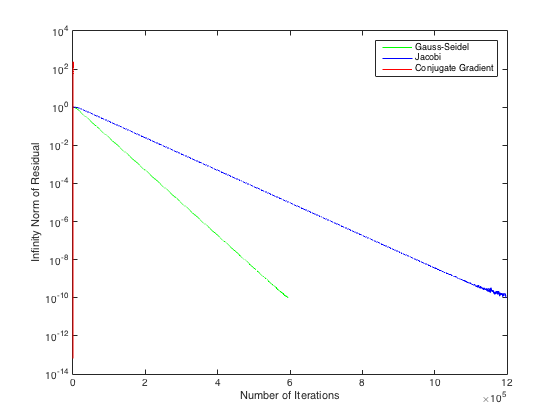
\includegraphics[scale=.7]{Figures/05_10_1.png}
        \end{center}

        We see in this plot that the Gauss-Seidel method converges much faster
        than either the Jacobi method or the Conjugate Gradient method.
        Looking at the slopes of these lines on the semilog plot, we can see that
        the Gauss-Seidel method converges quadractically while the Jacobi and
        Conjugate Gradient methods are converges linearly, this is visible because
        the slopes of these lines are -2 and -1 respectively.
\end{enumerate}
\end{document}
